\chapter{Espaces vectoriels normés}
\label{chap:evn}

\paragraph{Notations.} Dans tout ce chapitre, $K$ désigne $\mathbb{R}$ ou $\mathbb{C}$, muni de son module $|\cdot|$ (la valeur absolue si $K=\mathbb{R}$). L'hypothèse $K\in\{\mathbb{R},\mathbb{C}\}$ est essentielle : la définition d'une norme fait intervenir $|\lambda|$, et l'on utilise librement la relation d'ordre de $\mathbb{R}$. On suppose connues de première année les notions suivantes :
\begin{itemize}
\item espace vectoriel, sous-espace vectoriel, application linéaire (chapitre~\ref{chap:algebre-lineaire}) ;
\item la \textbf{propriété de la borne supérieure} de $\mathbb{R}$ : toute partie non vide et majorée de $\mathbb{R}$ admet une borne supérieure dans $\mathbb{R}$ ;
\item la droite réelle achevée $\overline{\mathbb{R}}=\mathbb{R}\cup\{-\infty,+\infty\}$, ainsi que les définitions
\[\lim_{n\to+\infty} u_n = +\infty \iff \forall A\in\mathbb{R},\ \exists N_0\in\mathbb{N},\ \forall n\geq N_0,\ u_n\geq A\]
et symétriquement pour $-\infty$ ;
\item la formule du binôme de Newton dans $\mathbb{R}$.
\end{itemize}

\section{Topologie dans un espace vectoriel normé}

\subsection{Normes et distances}

\begin{defi}[Norme]
\label{defi:norme}
Soit $E$ un $K$-espace vectoriel. On appelle \textbf{norme} sur $E$ toute application $N : E\to\mathbb{R}$ vérifiant :
\begin{enumerate}
\item \emph{(positivité)} $\forall x\in E,\ N(x)\geq 0$ ;
\item \emph{(séparation)} $\forall x\in E,\ N(x)=0 \implies x=0_E$ ;
\item \emph{(homogénéité)} $\forall\lambda\in K,\ \forall x\in E,\ N(\lambda x)=|\lambda|\,N(x)$ ;
\item \emph{(inégalité triangulaire)} $\forall x,y\in E,\ N(x+y)\leq N(x)+N(y)$.
\end{enumerate}
Un \textbf{espace vectoriel normé} (en abrégé : \textbf{e.v.n.}) est un couple $(E,N)$ où $N$ est une norme sur $E$. On note le plus souvent $N=\|\cdot\|$. Pour $x,y\in E$, la \textbf{distance} de $x$ à $y$ est
\[d(x,y) = \|x-y\|\]
\end{defi}

\begin{remarque}
Les axiomes 3 et 4 entraînent l'axiome 1, qui est donc redondant. En effet, l'homogénéité appliquée à $\lambda=0$ donne $N(0_E)=N(0\cdot 0_E)=|0|\,N(0_E)=0$ ; puis, pour $x\in E$,
\[0 = N(0_E) = N\big(x+(-x)\big) \leq N(x)+N(-x) = N(x)+|-1|\,N(x) = 2N(x)\]
d'où $N(x)\geq 0$. On garde néanmoins l'axiome 1 dans l'énoncé, conformément à l'usage.

Par ailleurs, la réciproque de l'axiome 2 est automatique : $N(0_E)=0$. On a donc bien $N(x)=0\iff x=0_E$.
\end{remarque}

\begin{exemple}
$(\mathbb{R},|\cdot|)$ et $(\mathbb{C},|\cdot|)$ sont des espaces vectoriels normés : les quatre axiomes sont les propriétés usuelles du module.
\end{exemple}

\begin{exemple}[Normes usuelles sur $K^n$]
\label{ex:normes-kn}
Soit $n\geq 1$. Pour $z=(z_1,\dots,z_n)\in K^n$, on pose
\[\|z\|_1 = \sum_{i=1}^{n}|z_i|, \qquad \|z\|_2 = \sqrt{\sum_{i=1}^{n}|z_i|^2}, \qquad \|z\|_\infty = \max_{1\leq i\leq n}|z_i|\]
Ce sont trois normes sur $K^n$.
\end{exemple}

\begin{proof}
Traitons $\|\cdot\|_1$ et $\|\cdot\|_\infty$ ; la démonstration de l'inégalité triangulaire pour $\|\cdot\|_2$ repose sur l'inégalité de Cauchy--Schwarz et est admise ici.

\textbf{Pour $\|\cdot\|_1$.}
\emph{Positivité :} c'est une somme finie de termes positifs.
\emph{Séparation :} supposons $\|z\|_1=0$. Pour tout $i$, $0\leq |z_i| \leq \sum_{j=1}^{n}|z_j| = 0$ (les autres termes étant positifs), donc $|z_i|=0$, donc $z_i=0$. Ainsi $z=0$.
\emph{Homogénéité :} $\|\lambda z\|_1 = \sum_{i=1}^n |\lambda z_i| = \sum_{i=1}^n |\lambda|\,|z_i| = |\lambda|\,\|z\|_1$.
\emph{Inégalité triangulaire :} pour tout $i$, $|z_i+z_i'|\leq |z_i|+|z_i'|$ ; en sommant ces $n$ inégalités,
\[\|z+z'\|_1 = \sum_{i=1}^{n}|z_i+z_i'| \leq \sum_{i=1}^{n}\big(|z_i|+|z_i'|\big) = \|z\|_1+\|z'\|_1\]

\textbf{Pour $\|\cdot\|_\infty$.} Le maximum existe : il porte sur un nombre fini ($n\geq 1$) de réels.
\emph{Positivité :} c'est un maximum de termes positifs.
\emph{Séparation :} si $\|z\|_\infty=0$, alors pour tout $i$, $0\leq|z_i|\leq\|z\|_\infty=0$, donc $z_i=0$.
\emph{Homogénéité :} comme $|\lambda|\geq 0$, la multiplication par $|\lambda|$ est croissante sur $\mathbb{R}$, donc
\[\|\lambda z\|_\infty = \max_{1\leq i\leq n}\big(|\lambda|\,|z_i|\big) = |\lambda|\max_{1\leq i\leq n}|z_i| = |\lambda|\,\|z\|_\infty\]
\emph{Inégalité triangulaire :} pour tout $i$,
\[|z_i+z_i'| \leq |z_i|+|z_i'| \leq \|z\|_\infty + \|z'\|_\infty\]
Le réel $\|z\|_\infty+\|z'\|_\infty$ majore donc les $n$ quantités $|z_i+z_i'|$, donc majore leur maximum :
\[\|z+z'\|_\infty \leq \|z\|_\infty+\|z'\|_\infty\qedhere\]
\end{proof}

\subsection{Boules et parties bornées}

Dans toute cette sous-section, $(E,\|\cdot\|)$ est un e.v.n., $a\in E$ et $r>0$.

\begin{defi}[Boules]
\label{defi:boule}
On appelle
\[B(a,r) = \big\{x\in E \ \big|\ \|x-a\|<r\big\} \qquad\text{\textbf{boule ouverte} de centre $a$ et de rayon $r$,}\]
\[\overline{B}(a,r) = \big\{x\in E \ \big|\ \|x-a\|\leq r\big\} \qquad\text{\textbf{boule fermée} de centre $a$ et de rayon $r$.}\]
\end{defi}

\begin{exemple}
Dans $(\mathbb{R},|\cdot|)$ : $B(a,r)=\,]a-r,a+r[$ et $\overline{B}(a,r)=[a-r,a+r]$.

Dans $\mathbb{R}^2$, la boule unité fermée $\overline{B}(0,1)$ dépend de la norme choisie : c'est le disque pour $\|\cdot\|_2$, le « losange » $|x|+|y|\leq 1$ pour $\|\cdot\|_1$, et le carré $[-1,1]^2$ pour $\|\cdot\|_\infty$.
\begin{center}
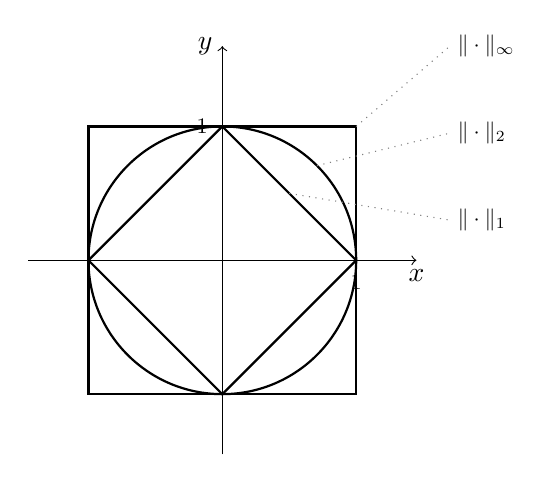
\begin{tikzpicture}[scale=1.7]
  \draw[->] (-1.45,0) -- (1.45,0) node[below] {$x$};
  \draw[->] (0,-1.45) -- (0,1.6) node[left] {$y$};
  \draw[thick] (-1,-1) rectangle (1,1);
  \draw[thick] (0,0) circle (1);
  \draw[thick] (1,0) -- (0,1) -- (-1,0) -- (0,-1) -- cycle;
  \draw (1,0.05) -- (1,-0.05) node[below,scale=0.8] {$1$};
  \draw (0.05,1) -- (-0.05,1) node[left,scale=0.8] {$1$};
  \draw[gray,dotted] (0.5,0.5) -- (1.7,0.3) node[right,scale=0.8,black] {$\|\cdot\|_1$};
  \draw[gray,dotted] (0.7071,0.7071) -- (1.7,0.95) node[right,scale=0.8,black] {$\|\cdot\|_2$};
  \draw[gray,dotted] (1,1) -- (1.7,1.6) node[right,scale=0.8,black] {$\|\cdot\|_\infty$};
\end{tikzpicture}
\end{center}
On observe l'emboîtement $\overline{B}_1(0,1)\subset\overline{B}_2(0,1)\subset\overline{B}_\infty(0,1)$, qui traduit les inégalités $\|z\|_\infty\leq\|z\|_2\leq\|z\|_1$.
\end{exemple}

\begin{defi}[Partie bornée]
\label{defi:borne}
Une partie $X\subset E$ est dite \textbf{bornée} s'il existe $C\in\mathbb{R}$ tel que
\[\forall x\in X,\quad \|x\|\leq C\]
autrement dit s'il existe $C$ tel que $X\subset\overline{B}(0_E,C)$.
\end{defi}

\begin{remarque}
Pour $E=\mathbb{R}$, on retrouve la définition usuelle : $X$ est bornée si et seulement s'il existe $m,M$ tels que $\forall x\in X,\ m\leq x\leq M$. En effet, une telle partie vérifie $|x|\leq\max(|m|,|M|)$ ; réciproquement $|x|\leq C$ donne $-C\leq x\leq C$.
\end{remarque}

\begin{prop}
\label{prop:boule-bornee}
Toute boule de $(E,\|\cdot\|)$ est bornée.
\end{prop}

\begin{proof}
Soient $a\in E$ et $r>0$. Posons $C=r+\|a\|$. Pour tout $x\in\overline{B}(a,r)$,
\[\|x\| = \|(x-a)+a\| \leq \|x-a\|+\|a\| \leq r+\|a\| = C\]
donc $\overline{B}(a,r)\subset\overline{B}(0,C)$ est bornée. Comme $B(a,r)\subset\overline{B}(a,r)$, la boule ouverte l'est aussi.
\end{proof}

\begin{defi}[Partie convexe]
\label{defi:convexe}
Une partie $C\subset E$ est dite \textbf{convexe} si
\[\forall x,y\in C,\ \forall t\in[0,1],\quad (1-t)x+ty \in C\]
\end{defi}

\begin{prop}
\label{prop:boule-convexe}
Les boules de $(E,\|\cdot\|)$ sont convexes.
\end{prop}

\begin{proof}
Soient $a\in E$, $r>0$, $x,y\in\overline{B}(a,r)$ et $t\in[0,1]$. Posons $z=(1-t)x+ty$. Comme $(1-t)+t=1$, on a $a=(1-t)a+ta$, donc
\[z-a = (1-t)(x-a)+t(y-a)\]
Comme $t\in[0,1]$, on a $|t|=t$ et $|1-t|=1-t$, d'où
\[\|z-a\| \leq (1-t)\|x-a\| + t\|y-a\| \leq (1-t)r+tr = r\]
donc $z\in\overline{B}(a,r)$.

Si $x,y\in B(a,r)$, la même majoration donne $\|z-a\|\leq(1-t)\|x-a\|+t\|y-a\|$. Si $t\in\,]0,1[$, les deux coefficients sont strictement positifs et les deux inégalités $\|x-a\|<r$, $\|y-a\|<r$ sont strictes, donc $\|z-a\|<r$. Si $t=0$ (resp. $t=1$), $z=x$ (resp. $z=y$) appartient à $B(a,r)$. Dans tous les cas $z\in B(a,r)$.
\end{proof}

\subsection{Voisinages, ouverts et fermés}

Dans toute cette sous-section, $(E,\|\cdot\|)$ est un e.v.n.

\begin{defi}[Voisinage]
\label{defi:voisinage}
Soit $a\in E$. Une partie $V\subset E$ est un \textbf{voisinage} de $a$ s'il existe $r>0$ tel que
\[B(a,r)\subset V\]
\end{defi}

\begin{defi}[Ouvert, fermé]
\label{defi:ouvert}
Une partie $O\subset E$ est un \textbf{ouvert} de $E$ si elle est voisinage de chacun de ses points :
\[\forall x\in O,\ \exists r_x>0,\quad B(x,r_x)\subset O\]
Une partie $W\subset E$ est un \textbf{fermé} de $E$ si son complémentaire $E\setminus W$ est un ouvert de $E$.
\end{defi}

\begin{remarque}
« Fermé » n'est pas la négation de « ouvert » : une partie peut être les deux à la fois (proposition~\ref{prop:vide-plein}) ou ni l'un ni l'autre (par exemple $[0,1[$ dans $\mathbb{R}$).
\end{remarque}

\begin{prop}
\label{prop:vide-plein}
$\varnothing$ et $E$ sont à la fois des ouverts et des fermés de $E$.
\end{prop}

\begin{proof}
$E$ est ouvert : pour $x\in E$, $B(x,1)\subset E$. $\varnothing$ est ouvert : la condition « $\forall x\in\varnothing,\dots$ » est vraie par vacuité. Comme $E\setminus\varnothing=E$ et $E\setminus E=\varnothing$ sont ouverts, $\varnothing$ et $E$ sont aussi fermés.
\end{proof}

\begin{prop}
\label{prop:boules-ouvert-ferme}
Toute boule ouverte est un ouvert de $E$ ; toute boule fermée est un fermé de $E$.
\end{prop}

\begin{proof}
\textbf{Boule ouverte.} Soient $a\in E$, $r>0$ et $x\in B(a,r)$. Posons $\rho=r-\|x-a\|$ ; comme $\|x-a\|<r$, on a $\rho>0$. Montrons $B(x,\rho)\subset B(a,r)$. Soit $y\in B(x,\rho)$ :
\[\|y-a\| = \|(y-x)+(x-a)\| \leq \|y-x\|+\|x-a\| < \rho + \|x-a\| = r\]
donc $y\in B(a,r)$. Ainsi $B(a,r)$ est voisinage de chacun de ses points.

\textbf{Boule fermée.} Soient $a\in E$, $R>0$. Montrons que $E\setminus\overline{B}(a,R)$ est un ouvert. Soit $x\notin\overline{B}(a,R)$, c'est-à-dire $\|x-a\|>R$. Posons $\rho=\|x-a\|-R>0$ et montrons $B(x,\rho)\subset E\setminus\overline{B}(a,R)$. Soit $y\in B(x,\rho)$. L'inégalité triangulaire donne
\[\|x-a\| \leq \|x-y\|+\|y-a\| < \rho+\|y-a\|\]
donc $\|y-a\| > \|x-a\|-\rho = R$, c'est-à-dire $y\notin\overline{B}(a,R)$.
\end{proof}

\begin{prop}
\label{prop:union-ouverts}
Soit $(O_i)_{i\in I}$ une famille d'ouverts de $E$.
\begin{enumerate}
\item $\displaystyle\bigcup_{i\in I} O_i$ est un ouvert de $E$ (réunion \emph{quelconque}).
\item Si $I$ est \emph{fini}, $\displaystyle\bigcap_{i\in I} O_i$ est un ouvert de $E$ (intersection \emph{finie}).
\end{enumerate}
\end{prop}

\begin{proof}
\textbf{1.} Soit $x\in\bigcup_{i\in I}O_i$ : il existe $i_0\in I$ tel que $x\in O_{i_0}$. Comme $O_{i_0}$ est ouvert, il existe $r>0$ tel que $B(x,r)\subset O_{i_0}\subset\bigcup_{i\in I}O_i$.

\textbf{2.} Si $I=\varnothing$, l'intersection vaut $E$, qui est ouvert. Sinon, écrivons $I=\inter{1}{m}$ et soit $x\in\bigcap_{i=1}^{m}O_i$. Pour chaque $i$, $x\in O_i$ ouvert, donc il existe $r_i>0$ tel que $B(x,r_i)\subset O_i$. Posons
\[\rho = \min(r_1,\dots,r_m)\]
Ce minimum existe (famille finie non vide) et $\rho>0$ comme minimum d'un nombre fini de réels strictement positifs. Pour tout $i$, $B(x,\rho)\subset B(x,r_i)\subset O_i$, donc $B(x,\rho)\subset\bigcap_{i=1}^{m}O_i$.
\end{proof}

\begin{remarque}
L'hypothèse de finitude au point 2 est indispensable : dans $\mathbb{R}$,
\[\bigcap_{n\geq 1}\ \left]-\tfrac{1}{n},\tfrac{1}{n}\right[ \ = \ \{0\}\]
En effet $0$ appartient à tous ces intervalles ; et si $x\neq 0$, en choisissant $n\geq 1/|x|$ on obtient $1/n\leq|x|$, donc $x\notin\,]-1/n,1/n[$. Or $\{0\}$ n'est pas un ouvert de $\mathbb{R}$ : aucune boule $]-r,r[$ avec $r>0$ n'est incluse dans $\{0\}$.
\end{remarque}

\begin{coro}
\label{coro:fermes}
Soit $(W_i)_{i\in I}$ une famille de fermés de $E$.
\begin{enumerate}
\item $\displaystyle\bigcap_{i\in I} W_i$ est un fermé de $E$ (intersection \emph{quelconque}).
\item Si $I$ est \emph{fini}, $\displaystyle\bigcup_{i\in I} W_i$ est un fermé de $E$ (réunion \emph{finie}).
\end{enumerate}
\end{coro}

\begin{proof}
Par passage au complémentaire. Les lois de De Morgan donnent
\[E\setminus\bigcap_{i\in I}W_i = \bigcup_{i\in I}\big(E\setminus W_i\big), \qquad E\setminus\bigcup_{i\in I}W_i = \bigcap_{i\in I}\big(E\setminus W_i\big)\]
Chaque $E\setminus W_i$ est un ouvert par définition d'un fermé. Le premier membre de droite est donc un ouvert (réunion quelconque d'ouverts), et le second l'est aussi lorsque $I$ est fini, d'après la proposition~\ref{prop:union-ouverts}.
\end{proof}

\begin{remarque}
Là encore, la finitude est nécessaire au point 2 : dans $\mathbb{R}$,
\[\bigcup_{n\geq 2}\left[-1+\tfrac1n,\ 1-\tfrac1n\right] = \,]-1,1[\]
(chaque segment est inclus dans $]-1,1[$ ; réciproquement, si $|x|<1$, tout $n\geq \max\big(2,\tfrac{1}{1-|x|}\big)$ convient). Or $]-1,1[$ n'est pas un fermé de $\mathbb{R}$ : son complémentaire $]-\infty,-1]\cup[1,+\infty[$ n'est pas ouvert, car toute boule $]1-r,1+r[$ rencontre $]-1,1[$.
\end{remarque}

\subsection{Espaces produits}

\begin{prop}[Norme produit]
\label{prop:norme-produit}
Soient $(E_1,\|\cdot\|_1),\dots,(E_m,\|\cdot\|_m)$ des e.v.n. sur un même corps $K$, et $F=E_1\times\dots\times E_m$ muni de sa structure de $K$-espace vectoriel produit. Alors
\[\|(x_1,\dots,x_m)\|_F = \max_{1\leq i\leq m}\|x_i\|_i\]
définit une norme sur $F$.
\end{prop}

\begin{proof}
Identique à celle donnée pour $\|\cdot\|_\infty$ sur $K^n$ (exemple~\ref{ex:normes-kn}), en remplaçant $|z_i|$ par $\|x_i\|_i$ :
\emph{positivité} et \emph{séparation} car $\|x\|_F=0$ force $\|x_i\|_i=0$ donc $x_i=0_{E_i}$ pour tout $i$ ;
\emph{homogénéité} car $\|\lambda x\|_F=\max_i\big(|\lambda|\,\|x_i\|_i\big)=|\lambda|\max_i\|x_i\|_i$ ;
\emph{inégalité triangulaire} car pour tout $i$, $\|x_i+y_i\|_i\leq\|x_i\|_i+\|y_i\|_i\leq\|x\|_F+\|y\|_F$, et ce majorant commun majore donc le maximum.
\end{proof}

\begin{remarque}
Sauf mention contraire, un produit fini d'e.v.n. est toujours muni de cette norme. En particulier, $K^n=K\times\dots\times K$ est par défaut muni de $\|\cdot\|_\infty$.
\end{remarque}

\section{Suites réelles}

\subsection{Suites monotones}

\begin{defi}
\label{defi:suite-monotone}
Soit $(u_n)_{n\in\mathbb{N}}\in\mathbb{R}^{\mathbb{N}}$. On dit que $(u_n)$ est
\begin{itemize}
\item \textbf{croissante} si $\forall n\in\mathbb{N},\ u_n\leq u_{n+1}$ ;
\item \textbf{décroissante} si $(-u_n)_{n\in\mathbb{N}}$ est croissante, c'est-à-dire si $\forall n\in\mathbb{N},\ u_{n+1}\leq u_n$ ;
\item \textbf{monotone} si elle est croissante ou décroissante.
\end{itemize}
\end{defi}

\begin{remarque}
Une récurrence immédiate montre que si $(u_n)$ est croissante, alors $u_p\leq u_n$ dès que $p\leq n$.
\end{remarque}

\begin{theo}[Limite monotone]
\label{theo:limite-monotone}
Toute suite réelle monotone et bornée est convergente. Plus précisément :
\begin{itemize}
\item si $(u_n)$ est croissante et majorée, alors $(u_n)$ converge et $\displaystyle\lim_{n\to+\infty}u_n=\sup_{n\in\mathbb{N}}u_n$ ;
\item si $(u_n)$ est décroissante et minorée, alors $(u_n)$ converge et $\displaystyle\lim_{n\to+\infty}u_n=\inf_{n\in\mathbb{N}}u_n$.
\end{itemize}
\end{theo}

\begin{proof}
Supposons $(u_n)$ croissante et majorée par $M$. L'ensemble
\[A = \{u_n \mid n\in\mathbb{N}\}\]
est une partie de $\mathbb{R}$ non vide (elle contient $u_0$) et majorée par $M$. Par la propriété de la borne supérieure, $A$ admet une borne supérieure $\ell=\sup A\in\mathbb{R}$.

Soit $\varepsilon>0$. Comme $\ell$ est le \emph{plus petit} des majorants de $A$ et que $\ell-\varepsilon<\ell$, le réel $\ell-\varepsilon$ n'est pas un majorant de $A$ : il existe $n_0\in\mathbb{N}$ tel que
\[\ell-\varepsilon < u_{n_0}\]
Pour tout $n\geq n_0$, la croissance donne $u_{n_0}\leq u_n$, et $\ell$ majore $A$ donc $u_n\leq\ell$. Ainsi
\[\forall n\geq n_0,\qquad \ell-\varepsilon < u_{n_0}\leq u_n\leq\ell \implies |u_n-\ell|\leq\varepsilon\]
Ceci vaut pour tout $\varepsilon>0$ : $(u_n)$ converge vers $\ell=\sup_{n}u_n$.

Le cas décroissant s'en déduit en appliquant ce qui précède à $(-u_n)$, qui est croissante et majorée par $-m$ si $m$ minore $(u_n)$ : $(-u_n)$ converge vers $\sup_n(-u_n)=-\inf_n u_n$, donc $(u_n)$ converge vers $\inf_n u_n$.
\end{proof}

\begin{coro}
\label{coro:limite-monotone-rbar}
Toute suite réelle monotone admet une limite dans $\overline{\mathbb{R}}$. Précisément, si $(u_n)$ est croissante :
\[\lim_{n\to+\infty}u_n = \begin{cases} \sup_{n}u_n\in\mathbb{R} & \text{si } (u_n) \text{ est majorée,}\\[2pt] +\infty & \text{sinon.}\end{cases}\]
\end{coro}

\begin{proof}
Le cas majoré est le théorème~\ref{theo:limite-monotone}. Supposons $(u_n)$ croissante et non majorée. La négation de « $\exists M\in\mathbb{R},\ \forall n,\ u_n\leq M$ » s'écrit
\[\forall M\in\mathbb{R},\ \exists n_0\in\mathbb{N},\quad u_{n_0}>M\]
Soit $M\in\mathbb{R}$ et $n_0$ associé. Par croissance, pour tout $n\geq n_0$, $u_n\geq u_{n_0}>M$. C'est exactement la définition de $u_n\to+\infty$.

Le cas décroissant se déduit du cas croissant par passage à $(-u_n)$.
\end{proof}

\subsection{Théorèmes de comparaison et d'encadrement}

\begin{prop}[Comparaison]
\label{prop:comparaison}
Soient $(u_n)$ et $(v_n)$ deux suites réelles telles que $u_n\leq v_n$ pour tout $n$.
\begin{enumerate}
\item Si $u_n\xrightarrow[n\to+\infty]{}+\infty$, alors $v_n\xrightarrow[n\to+\infty]{}+\infty$.
\item Si $v_n\xrightarrow[n\to+\infty]{}-\infty$, alors $u_n\xrightarrow[n\to+\infty]{}-\infty$.
\end{enumerate}
\end{prop}

\begin{proof}
\textbf{1.} Soit $A\in\mathbb{R}$. Comme $u_n\to+\infty$, il existe $N_0$ tel que $\forall n\geq N_0,\ u_n\geq A$. Alors pour tout $n\geq N_0$, $v_n\geq u_n\geq A$. Donc $v_n\to+\infty$.

\textbf{2.} Soit $A\in\mathbb{R}$. Il existe $N_0$ tel que $\forall n\geq N_0,\ v_n\leq A$, donc $u_n\leq v_n\leq A$. Donc $u_n\to-\infty$.
\end{proof}

\begin{theo}[Théorème d'encadrement, dit « des gendarmes »]
\label{theo:gendarmes}
Soient $(u_n),(v_n),(w_n)$ trois suites réelles telles que
\[\forall n\in\mathbb{N},\quad u_n\leq v_n\leq w_n\]
Si $(u_n)$ et $(w_n)$ convergent vers une même limite $\ell\in\mathbb{R}$, alors $(v_n)$ converge et $\lim v_n=\ell$.
\end{theo}

\begin{proof}
Soit $\varepsilon>0$. Comme $u_n\to\ell$, il existe $n_1$ tel que $\forall n\geq n_1,\ |u_n-\ell|\leq\varepsilon$, donc en particulier $\ell-\varepsilon\leq u_n$. Comme $w_n\to\ell$, il existe $n_2$ tel que $\forall n\geq n_2,\ w_n\leq\ell+\varepsilon$. Alors, pour tout $n\geq\max(n_1,n_2)$,
\[\ell-\varepsilon \leq u_n \leq v_n \leq w_n \leq \ell+\varepsilon\]
c'est-à-dire $|v_n-\ell|\leq\varepsilon$. Donc $v_n\to\ell$.
\end{proof}

\subsection{Suites de référence}

\begin{prop}[Suites arithmétiques]
Soit $a\in\mathbb{R}$ et $(u_n)$ définie par $u_{n+1}=u_n+a$. Alors $u_n=u_0+na$ pour tout $n$, et
\[\lim_{n\to+\infty}u_n = \begin{cases} u_0 & \text{si } a=0,\\ +\infty & \text{si } a>0,\\ -\infty & \text{si } a<0.\end{cases}\]
\end{prop}

\begin{proof}
La formule $u_n=u_0+na$ s'obtient par récurrence immédiate. Si $a=0$ la suite est constante. Si $a>0$, pour $A\in\mathbb{R}$ et $n\geq (A-u_0)/a$ on a $u_n\geq A$, donc $u_n\to+\infty$ ; le cas $a<0$ s'en déduit en considérant $(-u_n)$.
\end{proof}

\begin{prop}[Suites géométriques]
\label{prop:suite-geometrique}
Soit $q\in\mathbb{R}$. La suite $(q^n)_{n\in\mathbb{N}}$ vérifie :
\begin{enumerate}
\item si $|q|<1$, alors $q^n\to 0$ ;
\item si $q=1$, alors $q^n\to 1$ (suite constante) ;
\item si $q>1$, alors $q^n\to+\infty$ ;
\item si $q\leq -1$, alors $(q^n)$ n'admet pas de limite dans $\overline{\mathbb{R}}$.
\end{enumerate}
En conséquence, la suite géométrique $u_n=q^n u_0$ converge vers $0$ si $|q|<1$, et est constante égale à $u_0$ si $q=1$.
\end{prop}

\begin{proof}
\textbf{3. Cas $q>1$.} Écrivons $q=1+\varepsilon$ avec $\varepsilon>0$. La formule du binôme donne
\[q^n = (1+\varepsilon)^n = \sum_{k=0}^{n}\binom{n}{k}\varepsilon^k = 1+n\varepsilon+\underbrace{\sum_{k=2}^{n}\binom{n}{k}\varepsilon^k}_{\geq 0}\ \geq\ 1+n\varepsilon\]
(inégalité de Bernoulli). Comme $1+n\varepsilon\to+\infty$, la proposition~\ref{prop:comparaison} donne $q^n\to+\infty$.

\textbf{1. Cas $|q|<1$.} Si $q=0$, la suite est nulle à partir du rang $1$. Sinon $0<|q|<1$, donc $1/|q|>1$ et, d'après le point 3, $(1/|q|)^n\to+\infty$. Soit $\varepsilon>0$ : en appliquant la définition avec $A=1/\varepsilon$, il existe $N_0$ tel que
\[\forall n\geq N_0,\quad \left(\frac{1}{|q|}\right)^{n}\geq\frac{1}{\varepsilon}\]
En passant aux inverses (tous les termes sont strictement positifs, et $x\mapsto 1/x$ est décroissante sur $\mathbb{R}_+^*$), $|q|^n\leq\varepsilon$, c'est-à-dire $|q^n-0|\leq\varepsilon$. Donc $q^n\to 0$.

\textbf{4. Cas $q=-1$.} Supposons par l'absurde que $((-1)^n)$ admette une limite $\ell\in\overline{\mathbb{R}}$. La suite étant bornée, $\ell\in\mathbb{R}$. Toute suite extraite converge alors vers $\ell$ ; or la suite extraite des indices pairs est constante égale à $1$, donc $\ell=1$, et celle des indices impairs est constante égale à $-1$, donc $\ell=-1$ : contradiction.

\textbf{Cas $q<-1$.} On a $q^2>1$, donc $(q^2)^n\to+\infty$ d'après le point 3. Ainsi
\[q^{2n}=(q^2)^n\xrightarrow[n\to+\infty]{}+\infty \qquad\text{et}\qquad q^{2n+1}=q\,(q^2)^n\xrightarrow[n\to+\infty]{}-\infty\]
puisque $q<0$. Deux suites extraites ayant des limites différentes dans $\overline{\mathbb{R}}$, $(q^n)$ n'admet pas de limite.
\end{proof}

\section{Suites d'un espace vectoriel normé}

Soit $(E,\|\cdot\|)$ un e.v.n. On note $E^{\mathbb{N}}$ l'ensemble des suites d'éléments de $E$ ; muni des opérations terme à terme, c'est un $K$-espace vectoriel.

\subsection{Suites convergentes}

\begin{defi}[Convergence]
\label{defi:convergence}
Soit $u=(u_n)_{n\in\mathbb{N}}\in E^{\mathbb{N}}$. On dit que $(u_n)$ \textbf{converge} vers $\ell\in E$ si
\[\forall\varepsilon>0,\ \exists N_0\in\mathbb{N},\ \forall n\geq N_0,\quad \|u_n-\ell\|\leq\varepsilon\]
Une suite est dite \textbf{convergente} s'il existe un tel $\ell$, et \textbf{divergente} sinon.
\end{defi}

\begin{remarque}
Remplacer « $\leq\varepsilon$ » par « $<\varepsilon$ » donne une définition équivalente : si la propriété vaut avec $\leq$ pour tout $\varepsilon>0$, elle vaut avec $<$ en l'appliquant à $\varepsilon/2$ ; la réciproque est immédiate.
\end{remarque}

\begin{remarque}
\label{rq:norme-suite-reelle}
En posant $\alpha_n=\|u_n-\ell\|$, on obtient une suite \emph{réelle} positive, et la définition ci-dessus s'écrit exactement $\alpha_n\to 0$. Autrement dit
\[u_n\xrightarrow[n\to+\infty]{}\ell \text{ dans } E \iff \|u_n-\ell\|\xrightarrow[n\to+\infty]{}0 \text{ dans } \mathbb{R}\]
C'est ce qui permet de ramener l'étude des suites d'un e.v.n. à celle des suites réelles.
\end{remarque}

\begin{prop}[Unicité de la limite]
\label{prop:unicite-limite}
Si $(u_n)$ converge, sa limite est unique. On la note alors $\displaystyle\lim_{n\to+\infty}u_n$.
\end{prop}

\begin{proof}
Supposons que $\ell_1$ et $\ell_2$ soient deux limites de $(u_n)$. Comme $E$ est normé, $\ell_1=\ell_2$ équivaut à $\|\ell_1-\ell_2\|=0$ (séparation) ; montrons cette égalité.

Soit $\varepsilon>0$. Il existe $N_1$ tel que $\forall n\geq N_1,\ \|u_n-\ell_1\|\leq\varepsilon$, et $N_2$ tel que $\forall n\geq N_2,\ \|u_n-\ell_2\|\leq\varepsilon$. Pour $n\geq\max(N_1,N_2)$ (un tel $n$ existe),
\[\|\ell_1-\ell_2\| = \|(\ell_1-u_n)+(u_n-\ell_2)\| \leq \|u_n-\ell_1\|+\|u_n-\ell_2\| \leq 2\varepsilon\]
Ainsi $\|\ell_1-\ell_2\|\leq 2\varepsilon$ pour tout $\varepsilon>0$. Or, pour $A\in\mathbb{R}$, si $A\leq 2\varepsilon$ pour tout $\varepsilon>0$ alors $A\leq 0$ : sinon $A>0$ et le choix $\varepsilon=A/4$ donnerait $A\leq A/2$, donc $A\leq 0$, absurde. Comme de plus $\|\ell_1-\ell_2\|\geq 0$, on conclut $\|\ell_1-\ell_2\|=0$.
\end{proof}

\begin{prop}
\label{prop:convergente-bornee}
Toute suite convergente de $E$ est bornée, c'est-à-dire que $\{u_n\mid n\in\mathbb{N}\}$ est une partie bornée de $E$.
\end{prop}

\begin{proof}
Soit $(u_n)$ convergeant vers $\ell$. En appliquant la définition avec $\varepsilon=1$, il existe $N_1\in\mathbb{N}$ tel que
\[\forall n\geq N_1,\quad \|u_n-\ell\|\leq 1\]
d'où, pour $n\geq N_1$,
\[\|u_n\| = \|(u_n-\ell)+\ell\| \leq \|u_n-\ell\|+\|\ell\| \leq 1+\|\ell\|\]
Posons $M=\max\big(\|u_0\|,\|u_1\|,\dots,\|u_{N_1}\|,\ 1+\|\ell\|\big)$, maximum d'un nombre \emph{fini} de réels. Alors $\|u_n\|\leq M$ pour tout $n\in\mathbb{N}$ : les indices $n<N_1$ sont couverts par les premiers termes du maximum, les indices $n\geq N_1$ par le dernier.
\end{proof}

\subsection{Théorèmes d'opérations}

\begin{prop}
\label{prop:somme-limites}
Soient $(u_n),(v_n)\in E^{\mathbb{N}}$ convergeant respectivement vers $\ell_1$ et $\ell_2$. Alors $(u_n+v_n)$ converge et
\[\lim_{n\to+\infty}(u_n+v_n) = \ell_1+\ell_2\]
\end{prop}

\begin{proof}
L'inégalité triangulaire donne, pour tout $n$,
\[\big\|(u_n+v_n)-(\ell_1+\ell_2)\big\| = \big\|(u_n-\ell_1)+(v_n-\ell_2)\big\| \leq \|u_n-\ell_1\|+\|v_n-\ell_2\|\]
Soit $\varepsilon>0$. Il existe $N_1$ tel que $\forall n\geq N_1,\ \|u_n-\ell_1\|\leq\varepsilon/2$, et $N_2$ tel que $\forall n\geq N_2,\ \|v_n-\ell_2\|\leq\varepsilon/2$. Pour $n\geq\max(N_1,N_2)$, la majoration ci-dessus donne
\[\big\|(u_n+v_n)-(\ell_1+\ell_2)\big\| \leq \frac{\varepsilon}{2}+\frac{\varepsilon}{2} = \varepsilon\qedhere\]
\end{proof}

\begin{prop}
\label{prop:scalaire-limite}
Soient $(u_n)\in E^{\mathbb{N}}$ convergeant vers $\ell$ et $\lambda\in K$. Alors $(\lambda u_n)$ converge et $\lim(\lambda u_n)=\lambda\ell$.
\end{prop}

\begin{proof}
Par homogénéité de la norme, $\|\lambda u_n-\lambda\ell\| = |\lambda|\,\|u_n-\ell\|$. Soit $\varepsilon>0$. Comme $|\lambda|+1>0$, il existe $N_0$ tel que
\[\forall n\geq N_0,\quad \|u_n-\ell\|\leq\frac{\varepsilon}{|\lambda|+1}\]
d'où $\|\lambda u_n-\lambda\ell\|\leq\dfrac{|\lambda|}{|\lambda|+1}\varepsilon\leq\varepsilon$. (On divise par $|\lambda|+1$ plutôt que par $|\lambda|$ pour traiter d'un coup le cas $\lambda=0$.)
\end{proof}

\begin{coro}
\label{coro:cv-sev}
L'ensemble $\mathcal{CV}(E)$ des suites convergentes de $E$ est un sous-espace vectoriel de $E^{\mathbb{N}}$, et l'application
\[\theta : \mathcal{CV}(E)\longrightarrow E, \qquad (u_n)_{n\in\mathbb{N}}\longmapsto \lim_{n\to+\infty}u_n\]
est linéaire.
\end{coro}

\begin{proof}
$\mathcal{CV}(E)$ contient la suite nulle (qui converge vers $0_E$), donc est non vide. Soient $(u_n),(v_n)\in\mathcal{CV}(E)$ de limites $\ell_1,\ell_2$ et $\lambda\in K$. D'après les propositions~\ref{prop:somme-limites} et~\ref{prop:scalaire-limite}, la suite $(\lambda u_n+v_n)$ converge vers $\lambda\ell_1+\ell_2$. Cela montre à la fois que $\mathcal{CV}(E)$ est stable par combinaison linéaire — donc est un sous-espace vectoriel — et que
\[\theta\big(\lambda(u_n)+(v_n)\big) = \lambda\ell_1+\ell_2 = \lambda\,\theta\big((u_n)\big)+\theta\big((v_n)\big)\]
c'est-à-dire que $\theta$ est linéaire. (L'application $\theta$ est bien définie grâce à l'unicité de la limite, proposition~\ref{prop:unicite-limite}.)
\end{proof}

\begin{defi}[Application bilinéaire]
\label{defi:bilineaire}
Soient $E,F,G$ des $K$-espaces vectoriels. Une application $B:E\times F\to G$ est dite \textbf{bilinéaire} si elle est linéaire en chacune de ses deux variables :
\begin{itemize}
\item $\forall x\in E$, l'application $B(x,\cdot) : F\to G,\ y\mapsto B(x,y)$ appartient à $\mathcal{L}(F,G)$ ;
\item $\forall y\in F$, l'application $B(\cdot,y) : E\to G,\ x\mapsto B(x,y)$ appartient à $\mathcal{L}(E,G)$.
\end{itemize}
\end{defi}

\begin{exemple}
Sont bilinéaires :
\begin{itemize}
\item la multiplication $K\times K\to K$, $(x,y)\mapsto xy$ ;
\item la loi externe $K\times E\to E$, $(\lambda,x)\mapsto \lambda x$ ;
\item le produit scalaire $E\times E\to\mathbb{R}$, $(x,y)\mapsto\langle x\mid y\rangle$, sur un espace préhilbertien réel ;
\item le produit matriciel $\mathcal{M}_n(K)\times\mathcal{M}_n(K)\to\mathcal{M}_n(K)$, $(A,B)\mapsto AB$ ; plus généralement, le produit $\mathcal{A}\times\mathcal{A}\to\mathcal{A}$ d'une $K$-algèbre $\mathcal{A}$ ;
\item le déterminant $K^2\times K^2\to K$, $\big((a,c),(b,d)\big)\mapsto \det\begin{pmatrix} a & b \\ c & d\end{pmatrix}=ad-bc$.
\end{itemize}
\end{exemple}

\begin{theo}
\label{theo:bilineaire-limite}
Soient $(E,\|\cdot\|_E)$, $(F,\|\cdot\|_F)$, $(G,\|\cdot\|_G)$ des e.v.n. et $B:E\times F\to G$ une application bilinéaire telle qu'il existe $M\geq 0$ vérifiant
\[\forall (x,y)\in E\times F,\qquad \|B(x,y)\|_G \leq M\,\|x\|_E\,\|y\|_F \qquad (\star)\]
Si $(x_n)\in E^{\mathbb{N}}$ converge vers $\ell_1$ et $(y_n)\in F^{\mathbb{N}}$ converge vers $\ell_2$, alors $\big(B(x_n,y_n)\big)_{n\in\mathbb{N}}$ converge et
\[\lim_{n\to+\infty}B(x_n,y_n) = B(\ell_1,\ell_2)\]
\end{theo}

\begin{proof}
En insérant le terme intermédiaire $B(\ell_1,y_n)$ puis en utilisant la bilinéarité (linéarité en la première variable pour le premier groupe, en la seconde pour le second) :
\[B(x_n,y_n)-B(\ell_1,\ell_2) = \underbrace{B(x_n,y_n)-B(\ell_1,y_n)}_{=\,B(x_n-\ell_1,\ y_n)} + \underbrace{B(\ell_1,y_n)-B(\ell_1,\ell_2)}_{=\,B(\ell_1,\ y_n-\ell_2)}\]
L'inégalité triangulaire dans $G$ puis $(\star)$ donnent
\[\big\|B(x_n,y_n)-B(\ell_1,\ell_2)\big\|_G \leq M\,\|x_n-\ell_1\|_E\,\|y_n\|_F + M\,\|\ell_1\|_E\,\|y_n-\ell_2\|_F\]
Majorons chacun des deux termes.

\emph{Second terme :} $M\|\ell_1\|_E$ est une constante et $\|y_n-\ell_2\|_F\to 0$ (remarque~\ref{rq:norme-suite-reelle}), donc ce terme tend vers $0$ (proposition~\ref{prop:scalaire-limite} appliquée dans $\mathbb{R}$).

\emph{Premier terme :} la suite $(y_n)$ étant convergente, elle est bornée (proposition~\ref{prop:convergente-bornee}) : il existe $M'\geq 0$ tel que $\|y_n\|_F\leq M'$ pour tout $n$. Donc
\[0 \leq M\,\|x_n-\ell_1\|_E\,\|y_n\|_F \leq M M'\,\|x_n-\ell_1\|_E\]
Comme $\|x_n-\ell_1\|_E\to 0$, le majorant tend vers $0$, et le théorème d'encadrement~\ref{theo:gendarmes} donne que ce terme tend vers $0$.

La somme des deux majorants tend donc vers $0$, et un dernier encadrement
\[0 \leq \big\|B(x_n,y_n)-B(\ell_1,\ell_2)\big\|_G \leq M\,\|x_n-\ell_1\|_E\,\|y_n\|_F + M\,\|\ell_1\|_E\,\|y_n-\ell_2\|_F \xrightarrow[n\to+\infty]{} 0\]
donne $\big\|B(x_n,y_n)-B(\ell_1,\ell_2)\big\|_G\to 0$, c'est-à-dire la convergence annoncée (remarque~\ref{rq:norme-suite-reelle}).
\end{proof}

\begin{remarque}
L'hypothèse $(\star)$ est vérifiée par tous les exemples ci-dessus : $|xy|\leq|x|\,|y|$ dans $K$ (avec $M=1$), $\|\lambda x\|=|\lambda|\,\|x\|$, $|\langle x\mid y\rangle|\leq\|x\|_2\|y\|_2$ (Cauchy--Schwarz), et $\|AB\|\leq n\,\|A\|_\infty\|B\|_\infty$ pour des matrices de $\mathcal{M}_n(K)$. On retrouve ainsi, comme cas particuliers du théorème~\ref{theo:bilineaire-limite}, que le produit de deux suites réelles (ou complexes) convergentes converge vers le produit des limites.
\end{remarque}
